\documentclass[12pt,letterpaper]{article}
\usepackage[utf8]{inputenc}
\usepackage[spanish]{babel}
\usepackage{graphicx}
\usepackage[left=2cm,right=2cm,top=2cm,bottom=2cm]{geometry}
\usepackage{graphicx} % figuras
% \usepackage{subfigure} % subfiguras
\usepackage{float} % para usar [H]
\usepackage{amsmath}
%\usepackage{txfonts}
\usepackage{stackrel} 
\usepackage{multirow}
\usepackage{enumerate} % enumerados
\renewcommand{\labelitemi}{$-$}
\renewcommand{\labelitemii}{$\cdot$}
% \author{}
% \title{Caratula}
\begin{document}

% Fancy Header and Footer
% \usepackage{fancyhdr}
% \pagestyle{fancy}
% \cfoot{}
% \rfoot{\thepage}
%

% \usepackage[hidelinks]{hyperref} % CREA HYPERVINCULOS EN INDICE

% \author{}
\title{Caratula}

\begin{titlepage}
	\begin{center}
	
	\begin{figure}[htb]
	\begin{center}
	
\includegraphics[width=4cm]{./Imagenes/UPT}
	\end{center}
	\end{figure}
	\vspace*{0.15in}
	\large{UNIVERSIDAD PRIVADA DE TACNA}\\
	\vspace*{0.10in}
	\large{Facultad de Ingeniería}\\
	\vspace*{0.10in}
	Escuela Profesional de Ingeniería de Sistemas  \\
	
\hfill \break
	
	\vspace*{0.1in}
	\begin{Large}
	\textbf{Práctica de Laboratorio N° 02: \\ Importación, Data Flow y Traslado de Archivos} \\
	\end{Large}
\hfill \break
	
	\vspace*{0.3in}
	\begin{Large}
	\textbf{Curso:} \\
	\end{Large}
	
	\vspace*{0.1in}
	\begin{large}
	INTELIGENCIA DE NEGOCIOS\\
	\end{large}
	
	\vspace*{0.3in}
	\begin{Large}
	\textbf{Docente:} \\
	\end{Large}
	
	\vspace*{0.1in}
	\begin{large}
	 Ing. Patrick Cuadros Quiroga\\
	\end{large}
	
	\vspace*{0.2in}
	\vspace*{0.1in}
	\begin{large}
	\textbf{Alumna:} \\
	\begin{flushleft}
	Estrella Palacios, Katherine Lizbeth	\hfill	(2016056193) 
	\end{flushleft}
	\end{large}

	\vspace*{0.5in}
	\begin{large}
	 Tacna - 2020\\
	\end{large}

	\end{center}

\end{titlepage}


\tableofcontents % INDICE
\thispagestyle{empty} % INDICE SIN NUMERO
\newpage
\setcounter{page}{1} % REINICIAR CONTADOR DE PAGINAS DESPUES DEL INDICE

%% ----------------------------------------------------------------------------------------------------------------------------------
\begin{center}
\begin{LARGE}
	\textbf{Práctica de Laboratorio N° 02: \\ Importación, Data Flow y Traslado de Archivos} \\ 
\end{LARGE}
\rule{175mm}{0.1mm}
\end{center}



%% ----------------------------------------------------------------------------------------------------------------------------------

\section{Objetivos}

\begin{itemize}
\item Importar datos usando el WIZARD 
\item Desarrollar mis primeros Paquetes DTSX

\end{itemize}

%% ----------------------------------------------------------------------------------------------------------------------------------
\section {\textbf{Requerimientos}}

\subsection{\textbf{Conocimientos}}
Para el desarrollo de esta práctica se requerirá de los siguientes conocimientos básicos:
\begin{itemize}
\item Conocimientos básicos de administración de base de datos Microsoft SQL Server.
\item Conocimientos básicos de SQL.
\end{itemize}



\subsection{\textbf{Software}}
Asimismo se necesita los siguientes aplicativos:
\begin{itemize}
\item SQL Server Integration Services
\item BD Adventure Work (OLTP y Data Warehouse)
\item BD AdventureWorkLT2012
\end{itemize}


	\begin{figure}[htb]
		\begin{center}
			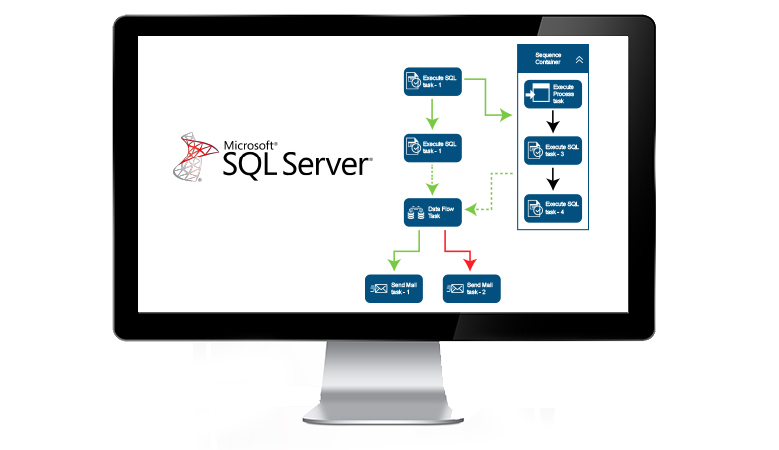
\includegraphics[width=13cm]{./IMAGENES/MS-SQL-Server-Integration-Services}
			
		\end{center}
	\end{figure}



%% ----------------------------------------------------------------------------------------------------------------------------------
\newpage

\section{Desarrollo}

%% TAREA 1-------------------------------------------------------------------------------------------------------------------

\subsection{TAREA N° 01: Importación de datos usando el WIZARD – SQL Managment}

\begin{itemize}
\item Crear una base de datos – BDTEST
	\begin{figure}[htb]
		\begin{center}
			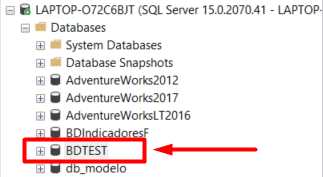
\includegraphics[width=8cm]{./IMAGENES/Tarea1_1}
			
		\end{center}
	\end{figure}
\item Importar Datos desde AdventureWorks
	\begin{figure}[htb]
		\begin{center}
			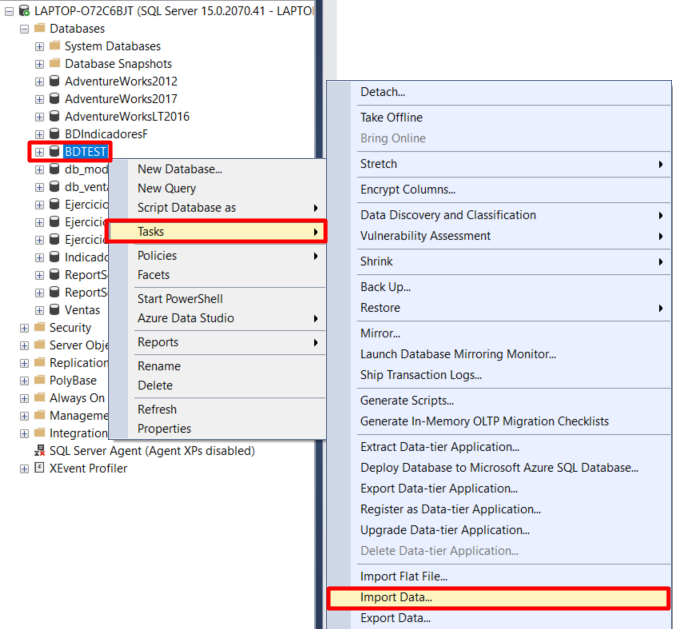
\includegraphics[width=13cm]{./IMAGENES/Tarea1_2}
			
		\end{center}
	\end{figure}

\newpage

\item Next y escribir el Servidor y seleccionar la base de datos
\item \textbf{Data Source:} La base de donde vamos a importar
\item \textbf{Destination:} La Base donde vamos a cargar la data
	\begin{figure}[htb]
		\begin{center}
			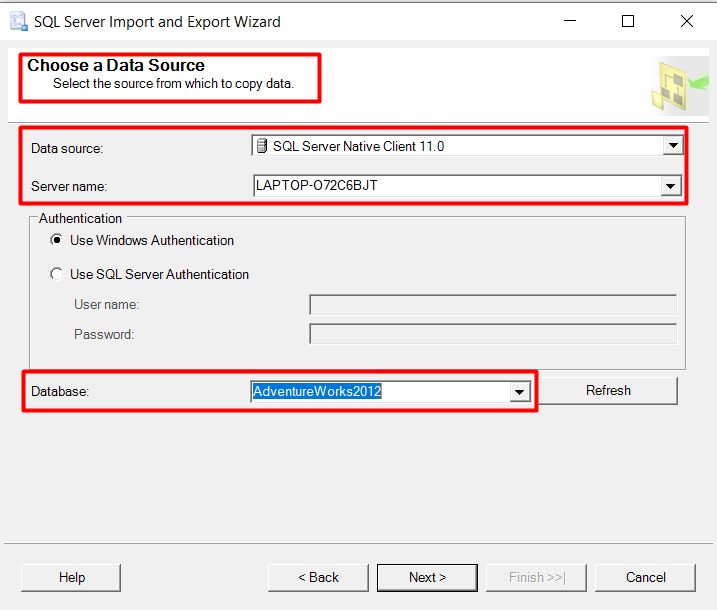
\includegraphics[width=8cm]{./IMAGENES/Tarea1_3}
			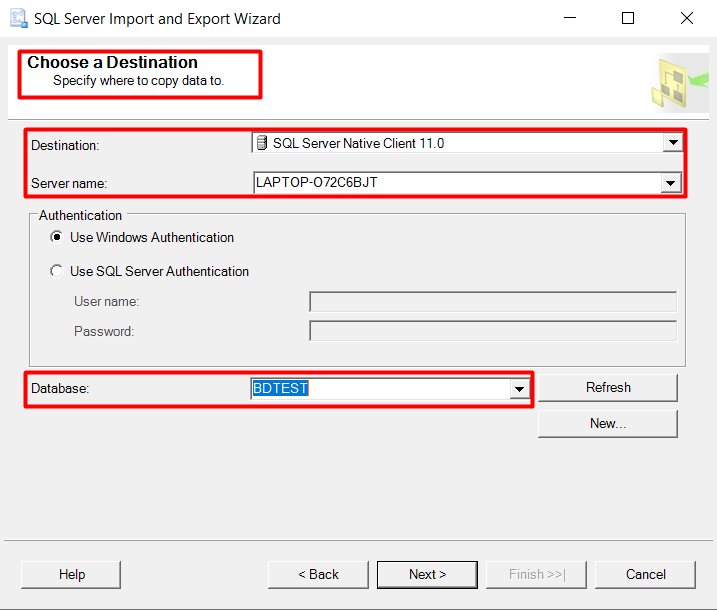
\includegraphics[width=8cm]{./IMAGENES/Tarea1_4}
		\end{center}
	\end{figure}

\item Podemos copiar los datos desde una o mas tablas o vistas. 
\item También podemos recuperar datos mediante una consulta SQL.
\item Seleccionamos: HumanResources.Department y Person.Address
	\begin{figure}[htb]
		\begin{center}
			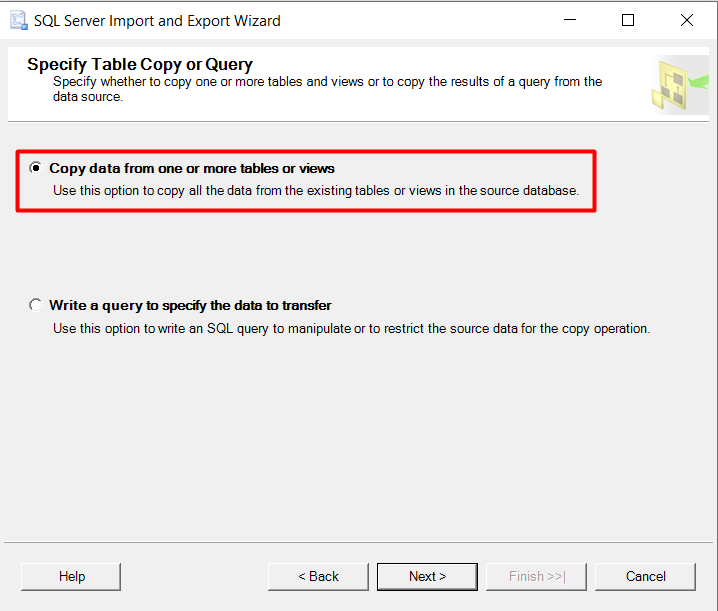
\includegraphics[width=8cm]{./IMAGENES/Tarea1_5}
			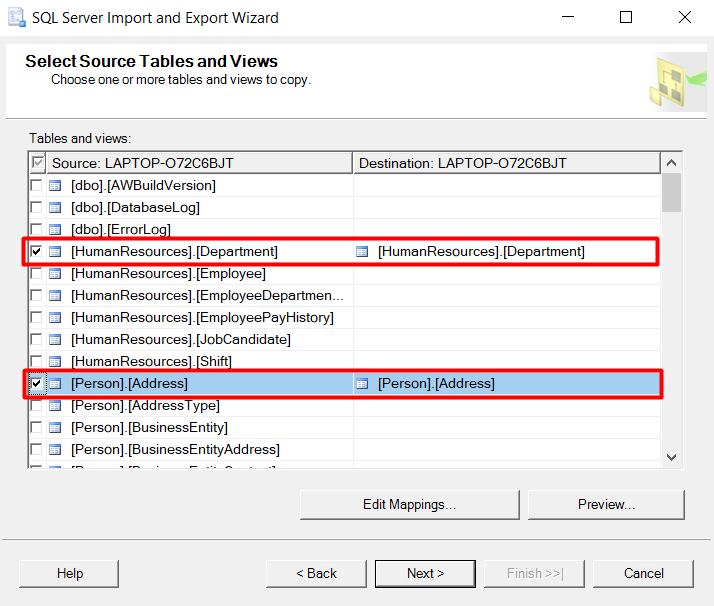
\includegraphics[width=8cm]{./IMAGENES/Tarea1_6}
		\end{center}
	\end{figure}

\newpage

\item Activamos para guardar el paquete.
\item Indicamos el lugar donde que va a guardar el DTSX.
	\begin{figure}[htb]
		\begin{center}
			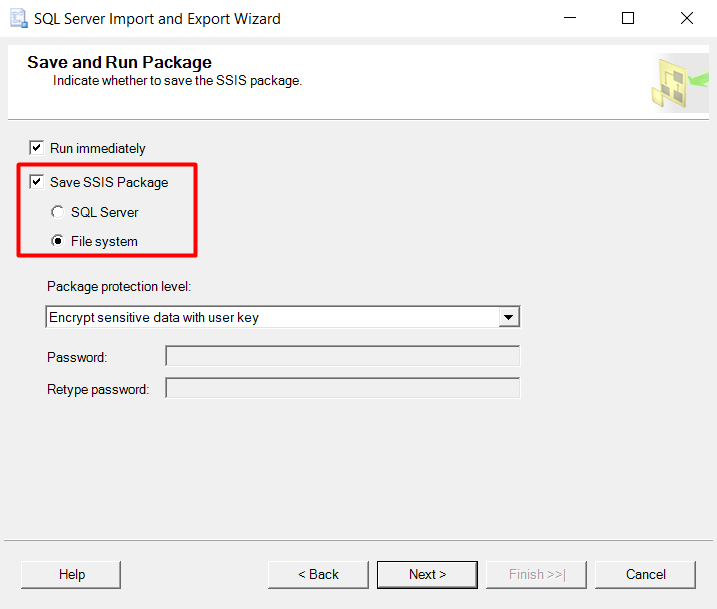
\includegraphics[width=8cm]{./IMAGENES/Tarea1_7}
			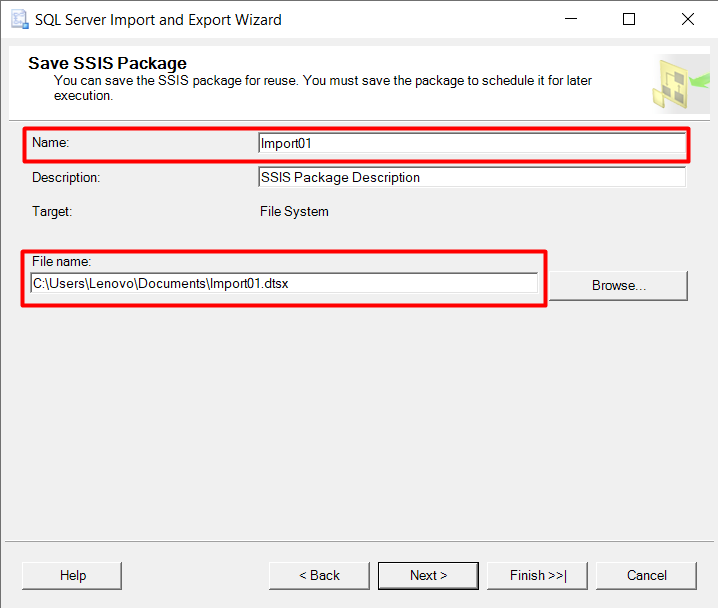
\includegraphics[width=8cm]{./IMAGENES/Tarea1_8}
		\end{center}
	\end{figure}



\item Le damos clic a Finalizar para completar las acciones.
\item Al finalizar tenemos el resumen de la ejecución
\item Hemos generado nuestro primer paquete de forma automática.
	\begin{figure}[htb]
		\begin{center}
			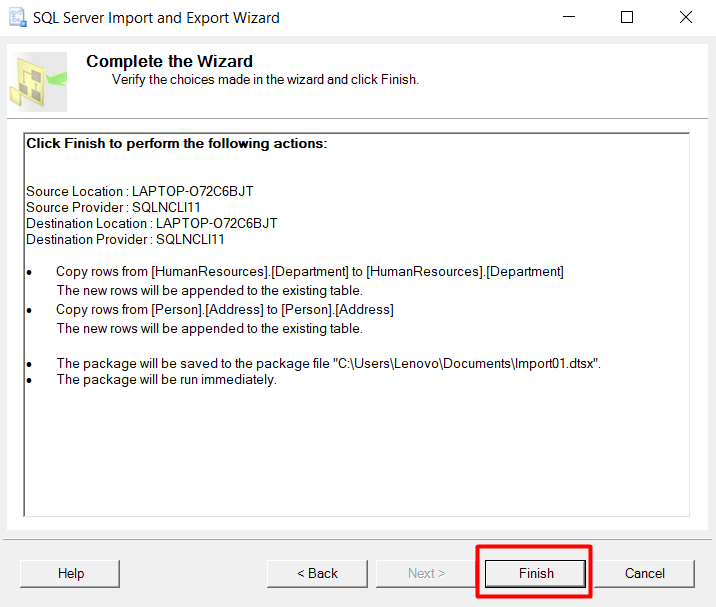
\includegraphics[width=8cm]{./IMAGENES/Tarea1_9}
			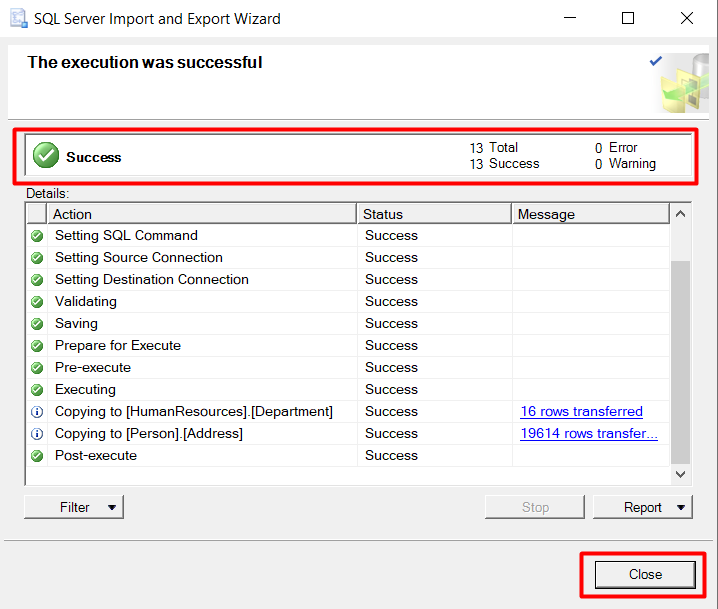
\includegraphics[width=8cm]{./IMAGENES/Tarea1_10}
		\end{center}
	\end{figure}

\newpage

\item Podemos actualizar la Base de Datos BDTEST y encontraremos las tablas ya importadas
	\begin{figure}[htb]
		\begin{center}
			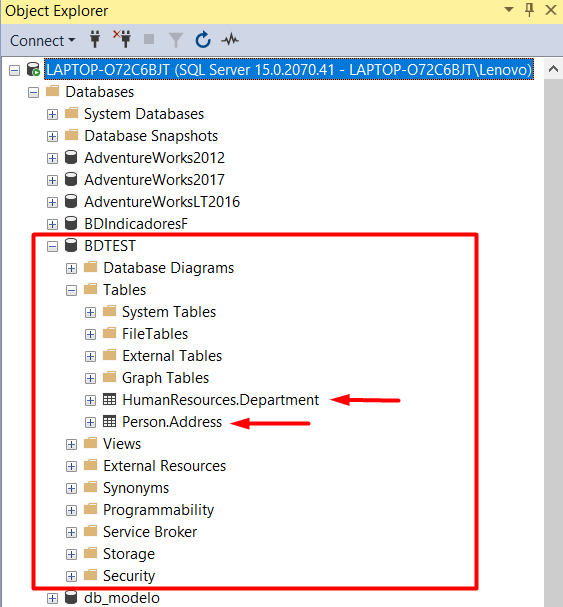
\includegraphics[width=12cm]{./IMAGENES/Tarea1_11}
		\end{center}
	\end{figure}

\end{itemize}

\newpage

%% TAREA 2-------------------------------------------------------------------------------------------------------------------

\subsection{TAREA N° 02: Creamos nuestro primer Paquete DTSX}

\begin{itemize}
\item Crear una base de datos – BDTEST
	\begin{figure}[htb]
		\begin{center}
			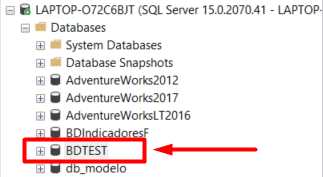
\includegraphics[width=8cm]{./IMAGENES/Tarea1_1}
			
		\end{center}
	\end{figure}
\item Importar Datos desde AdventureWorks
	\begin{figure}[htb]
		\begin{center}
			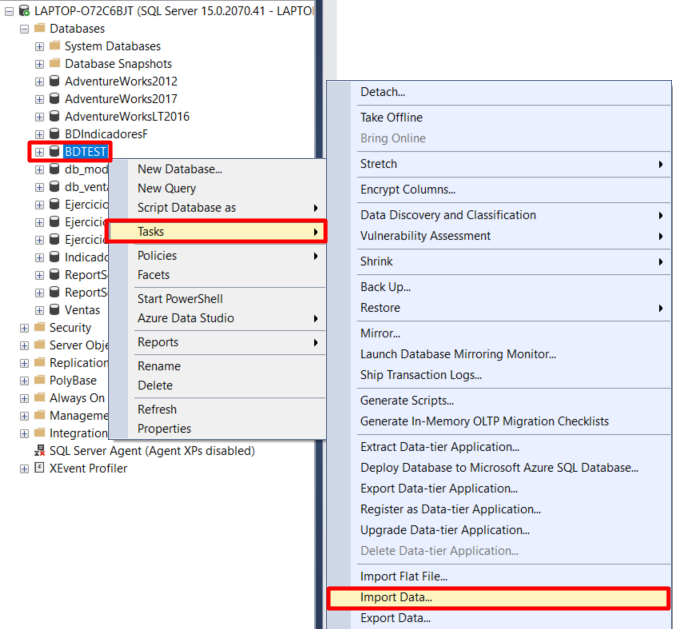
\includegraphics[width=13cm]{./IMAGENES/Tarea1_2}
			
		\end{center}
	\end{figure}

\newpage



\end{itemize}



\end{document}
